\documentclass[11pt,a4paper]{article}
\usepackage[utf8]{inputenc}
\usepackage{amsmath}
\usepackage{amsfonts}
\usepackage{amssymb}
\usepackage{graphicx}
\usepackage{mathtools}

\usepackage{listings}
\usepackage{color}
\definecolor{dkgreen}{rgb}{0,0.6,0}
\definecolor{gray}{rgb}{0.5,0.5,0.5}
\definecolor{mauve}{rgb}{0.58,0,0.82}

\lstset{frame=tb,
  language=Python,
  aboveskip=3mm,
  belowskip=3mm,
  showstringspaces=false,
  columns=flexible,
  basicstyle={\small\ttfamily},
  numbers=none,
  numberstyle=\tiny\color{gray},
  keywordstyle=\color{blue},
  commentstyle=\color{dkgreen},
  stringstyle=\color{mauve},
  breaklines=true,
  breakatwhitespace=true,
  tabsize=3
}



\newcommand{\qed}{\hfill $\blacksquare$}
\newcommand{\reals}{\mathbb{R}}
\newcommand{\complexes}{\mathbb{C}}
\author{Jacob Bruner}
\title{Perpetual Notes Document}

\begin{document}
\maketitle
\tableofcontents
\pagebreak

\iffalse
############
heres an example of a code block
\begin{lstlisting}
        def intervalValues(z, n):
            return output # return the sequence of values
\end{lstlisting}

heres an example of an image
\begin{figure}[h]
\begin{center}
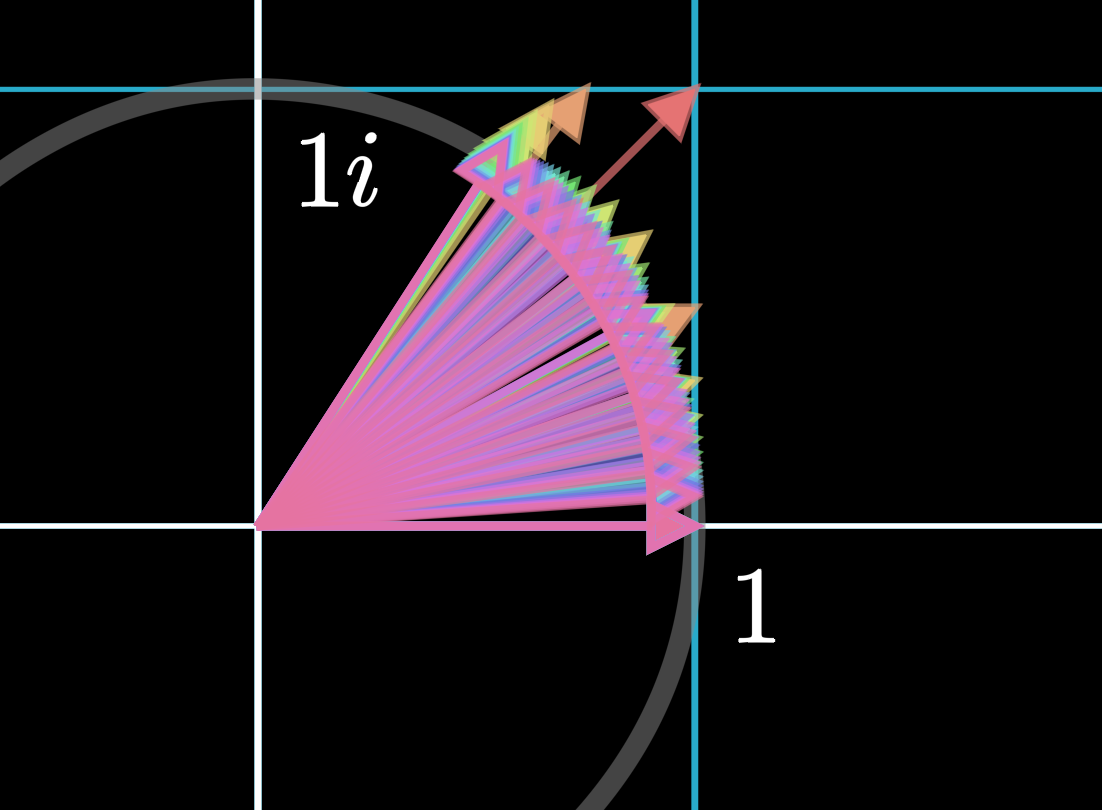
\includegraphics[scale=.37]{onefifteen} 
\caption{Sequences Generated by n = 1-15 on Argand Diagram}
\end{center}
\end{figure}
############
\fi

\section{Number Systems}
Suppose A is a 2-dim unital algebra over $\reals$.  \\
Consider: $B = \{ 1,  \alpha \}$,  \fbox{$x+y\alpha \in A$} \\
\textit{Note:} $\alpha \in A$ implies that $ \exists\  a,b \in \reals$ such that $ \alpha^2 = a+b \alpha$
\begin{align*}
&\Rightarrow \alpha^2 -bd = a \\
&\Rightarrow 4\alpha^2 - 4b\alpha + b^2 = 4a+b^2\\
&\Rightarrow (2\alpha-b)^2 = 4a + b^2 \in \reals
\end{align*}
This motivates another definition: \\
$B' = \{ 1, \beta \}$ where $\beta \coloneq 2 \alpha - b$, therefore $\beta^2 \in \reals$ \\

\underline{Case 1:} \\
\begin{align*}
\beta^2 = 0 \rightsquigarrow \text{set } \beta = \epsilon, \ \therefore \epsilon^2 = 0 \\
(a+b\epsilon)(c+d\epsilon) = ac+(ad+bc)\epsilon \\
A = \reals(\epsilon)
\end{align*}

\underline{Case 2:} \\
\begin{align*}
\beta^2 < 0 \rightsquigarrow \text{set } i = \frac{\beta}{|\beta^2|}, \ \therefore i^2 = -1 \\
(a+bi)(c+di) = (ac-bd)+(ad+bc)i \\
A = \complexes
\end{align*}

\underline{Case 3:} \\
\begin{align*}
\beta^2 > 0 \rightsquigarrow \text{set } j = \frac{\beta}{\beta^2}, \ \therefore j^2 = 1 \\
(a+bj)(c+dj) = (ac+bd)+(ad+bc)j \\
A = \reals(j) \\
\text{also} \cong \reals \times \reals
\end{align*}

\begin{align*}
e^{\pi i}=-1 \ ??? \\
^{\reals[x]}/_{x^2+1}\\ 
\hat{f} (w) = \int_{- \infty} ^{\infty} e^{-i w} f(t)dt \\
re^{i \theta} = r\cos(\theta) + ir\sin(\theta)
\end{align*}

'Complex' Numbers??
$
a+bi \cong \begin{pmatrix}
a & b \\
-b & a
\end{pmatrix}
$

\begin{align*}
\rho &= \frac{3.332\ g \ cm^{-1}}{\pi (\frac{1}{2}*1.25\ cm)^2} \\
\rho &= 2.715\ g \ cm^{-3}
\end{align*}
kj
\begin{align*}
\% u_{radius} &= \frac{\frac{1}{2}*0.05}{1.25}\\
\% u_{radius} &= 2\% 
\end{align*}

\begin{align*}
\%u_{total} &= 2*\% u_{radius} + \% u_{slope} \\
\%u_{total} &= 2*(2 \% ) + 6.18 \% \\
\%u_{total} &= 10.18 \%
\end{align*}

\begin{align*}
\rho = 2.72  \pm 0.28\  g\ cm^{-3}
\end{align*}

\end{document}
